\documentclass[12pt, titlepage]{article}

\usepackage{fullpage}
\usepackage[round]{natbib}
\usepackage{multirow}
\usepackage{booktabs}
\usepackage{tabularx}
\usepackage{graphicx}
\usepackage{float}
\usepackage{hyperref}
\hypersetup{
    colorlinks,
    citecolor=blue,
    filecolor=black,
    linkcolor=red,
    urlcolor=blue
}

%% Comments

\usepackage{color}

\newif\ifcomments\commentstrue %displays comments
%\newif\ifcomments\commentsfalse %so that comments do not display

\ifcomments
\newcommand{\authornote}[3]{\textcolor{#1}{[#3 ---#2]}}
\newcommand{\todo}[1]{\textcolor{red}{[TODO: #1]}}
\else
\newcommand{\authornote}[3]{}
\newcommand{\todo}[1]{}
\fi

\newcommand{\wss}[1]{\authornote{blue}{SS}{#1}} 
\newcommand{\plt}[1]{\authornote{magenta}{TPLT}{#1}} %For explanation of the template
\newcommand{\an}[1]{\authornote{cyan}{Author}{#1}}

%% Common Parts

\newcommand{\progname}{Scanalyze AI} % PUT YOUR PROGRAM NAME HERE
\newcommand{\authname}{Team 16, Ace
\\ Hamza Issa
\\ Ahmad Hamadi
\\ Jared Paul
\\ Gurnoor Bal} % AUTHOR NAMES                  

\usepackage{hyperref}
    \hypersetup{colorlinks=true, linkcolor=blue, citecolor=blue, filecolor=blue,
                urlcolor=blue, unicode=false}
    \urlstyle{same}
                                

\graphicspath{ {./} }

\newcounter{acnum}
\newcommand{\actheacnum}{AC\theacnum}
\newcommand{\acref}[1]{AC\ref{#1}}

\newcounter{ucnum}
\newcommand{\uctheucnum}{UC\theucnum}
\newcommand{\uref}[1]{UC\ref{#1}}

\newcounter{mnum}
\newcommand{\mthemnum}{M\themnum}
\newcommand{\mref}[1]{M\ref{#1}}

\begin{document}

\title{Module Guide for \progname{}} 
\author{\authname}
\date{\today}

\maketitle

\pagenumbering{roman}

\section{Revision History}

\begin{tabularx}{\textwidth}{p{3cm}p{2cm}X}
\toprule {\bf Date} & {\bf Version} & {\bf Notes}\\
\midrule
17 January & 1.0 & Finished MG \\
\bottomrule
\end{tabularx}

\newpage

\section{Reference Material}

This section records information for easy reference.

\subsection{Abbreviations and Acronyms}

\renewcommand{\arraystretch}{1.2}
\begin{tabular}{l l} 
  \toprule		
  \textbf{symbol} & \textbf{description}\\
  \midrule 
  AC & Anticipated Change\\
  DAG & Directed Acyclic Graph \\
  M & Module \\
  MG & Module Guide \\
  OS & Operating System \\
  R & Requirement\\
  SC & Scientific Computing \\
  SRS & Software Requirements Specification\\
  \progname & Explanation of program name\\
  UC & Unlikely Change \\
  \wss{etc.} & \wss{...}\\
  \bottomrule
\end{tabular}\\

\newpage

\tableofcontents

\listoftables

\listoffigures

\newpage

\pagenumbering{arabic}

\section{Introduction}

In order to build large scale software systems, the intended software system must be decomposed into smaller logical modules. Ideally, these modules should be independent and thus reusable across the software system or in the event of a future software change or a change in demand. This allows the software system to become resilient to unanticipated changes and more easily maintainable.

Following this approach, in developing a diffusion model to generate chest x-ray images, we will decompose the individual parts into clear single-responsibility modules. This will enable the software to be more maintainable and thus easier to update in the future in the face of changing demand or issues.

It is important that the CXR image data generated by this project are of high-quality such that if the quality is less than ideal it is completely unusable, and more so can result in damaging effects such as if the poor data was later used to train future machine learning models used in medicine.

As a result of this building this project in modular clear single responsibility components will enable us to continue to improve the accuracy of our model to ensure it continues to be usable in the future, such as making it easy to tune the model in accordance to new research findings or updating the software at large.
The purpose of this document is to explain how we’ve structured the system, why we made certain design choices, and how the parts of the system work together. It is intended to be useful for:

\begin{enumerate}
  \item Onboarding engineers: To easily introduce new engineers to the architecture of the software system in a digestible fashion.
  \item Future engineers: To enable future engineers to have clear documentation on how to proceed with their intended changes given the existing software architecture.
  \item Requirements engineers: To analyse the existing software architecture to reach a conclusion if the software meets the intended specifications and requirements.
\end{enumerate}

This design document aims to provide a structured and abstract explanation of the larger software architecture of this project. As a result, this document will include the large system design, single responsibility modules and the relationships between them.
The object is to ensure that future stakeholders and engineers can easily digest the architecture presented such that they may become capable to contribute to the project if necessary.


\section{Anticipated and Unlikely Changes} \label{SecChange}

This section outlines possible changes that may impact the system. These changes are categorized based on their likelihood: anticipated changes, which are expected and should be designed for, and unlikely changes, which are considered rare and would require significant modification to implement.


\subsection{Anticipated Changes} \label{SecAchange}

Anticipated changes are the areas of the system that are most likely to evolve and have been designed to accommodate future adjustments. Meaning that the software maintainability is built with this potential changes in mind. These changes are encapsulated within specific modules to ensure the system’s flexibility.

\begin{itemize}
  \item AC1: Model Architecture Updates:
  The architecture of the diffusion model may evolve as new research or improved techniques emerge. The system should support swapping or updating the model without significant rework.
  \item AC2 Chest X-ray Dataset Expansion:
  As more real-world chest X-ray datasets become available, the system should be able to integrate additional datasets for training or validation seamlessly.
  \item AC3 Synthetic Image Resolution:
  The resolution of the generated chest X-ray images may need to be increased or adjusted based on user requirements or advancements in computational resources.
  \item AC4 Evaluation Metrics:
  New evaluation metrics or benchmarks may be adopted to assess the quality of the generated images. The system should allow the addition of new evaluation pipelines.
  \item AC5 Export Formats for Generated Data:
  Users may require the generated chest X-rays in additional formats (e.g., DICOM, JPEG). The system should accommodate exporting in various formats.
  \item AC6 Integration with External Tools:
  The system may need to integrate with external tools, such as machine learning pipelines, medical imaging software, or hospital IT systems, to streamline usage.
\end{itemize}

\subsection{Unlikely Changes} \label{SecUchange}

Unlikely changes are those that would require significant rework and are considered fixed for the foreseeable future. Designing for these changes would add unnecessary complexity to the system.

\begin{itemize}
\item UC1 Core Diffusion Model Methodology:
A fundamental shift away from the diffusion model approach is considered highly unlikely, as it forms the core of the system's design.
\item UC2 Removal of Synthetic Data Generation:
Generating synthetic chest X-ray data is the primary purpose of the system. Removing this feature would negate the system’s value.
\item UC3 Elimination of GPU/TPU Acceleration:
Hardware acceleration (e.g., GPUs or TPUs) is critical for training and generating high-quality images efficiently. Moving to CPU-only processing is not expected.
\item UC4 Discontinuation of Medical Imaging Focus:
The system is tailored for medical imaging, specifically chest X-rays. A shift to a completely different domain is not anticipated.
\item UC5 Input Data Format Changes:
The system is designed to process standardized chest X-ray input formats (e.g., DICOM). A fundamental change in these formats is unlikely in the short term.
\item UC6 Standalone Usage Elimination:
The software is intended to be a standalone tool for generating and exporting chest X-rays. Transitioning to a fully dependent cloud-based or third-party service is not planned.
\end{itemize}

\section{Module Hierarchy} \label{SecMH}

This section of the document describes the modules that make up the project and their related hierarchy. Table 1 categorizes the modules based on encapsulation, whereas Table 2 categorizes modules according to the MVC architecture. Each category can be identified as nodes in a tree, where each of the respective modules in each category are leaves of that node.

Total Module List:
\begin{itemize}
  \item M1: DataPreprocessing Module
  \item M2: DiffusionModel Module
  \item M3: SyntheticImageGen Module
  \item M4: DatasetHandler Module
  \item M5: EvaluationMetrics Module
  \item M6: ImageExport Module
  \item M7: UserInterface Module
  \item M8: IntegrationModule (for external tools)
  \item M9: HardwareAcceleration Module
  \item M10: LoggingAndMonitoring Module
  \item M11: Login Module
\end{itemize}

\textbf{Table 1: Encapsulation}
\begin{table}[H]
  \begin{tabular}{lllll}
  \multicolumn{1}{c}{\textbf{Node}} & \multicolumn{1}{c}{\textbf{Leaf}} &  &  &  \\
  \textbf{Hardware Encapsulation} & HardwareAcceleration &  &  &  \\
  \textbf{Behavior Encapsulation} & DataPreprocessing, SyntheticImageGen, DatasetHandler, EvaluationMetrics, LoggingAndMonitoring, Login &  &  &  \\
  \textbf{Software Decision Encapsulation} & DiffusionModel, ImageExport, UserInterface, IntegrationModule &  &  & 
  \end{tabular}
\end{table}

\textbf{Table 2: Model-View Controller}
\begin{table}[H]
  \begin{tabular}{lllll}
  \multicolumn{1}{c}{\textbf{Node}} & \multicolumn{1}{c}{\textbf{Leaf}} &  &  &  \\
  \textbf{Model Module} & DataPreprocessing, DatasetHandler, SyntheticImageGen, EvaluationMetrics, UserAuthMgmt &  &  &  \\
  \textbf{View Module} & UserInterface, Login &  &  &  \\
  \textbf{Controller Module} & DiffusionModel, ImageExport, IntegrationModule, LoggingAndMonitoring &  &  & 
  \end{tabular}
\end{table}

\section{Connection Between Requirements and Design} \label{SecConnection}
Refer to Table 2

\section{Module Decomposition} \label{SecMD}

The structure of the system is based on the modular design principles outlined by David Parnas, which emphasize breaking down a system into independent components that hide their internal details. This ensures that changes made to one module do not unnecessarily affect others, leading to better maintainability and adaptability.

Each module encapsulates a specific "secret," or design decision, which represents the part of the system that is most likely to change. By isolating these secrets within modules, the software can more easily adapt to evolving requirements and unforeseen modifications. The Services field describes the functionality of the module at a high level, while the Implemented By field specifies the responsible implementation mechanism. Only the "leaf" modules, those at the end of the hierarchy, are developed and implemented directly.

This modular approach allows for clear boundaries between components, ensuring that the overall system remains flexible and scalable. The following subsections detail each module's secrets, services, and implementation specifics.

\subsection{Hardware Hiding Modules (\mref{mHH})}

Secrets: The data structure and algorithm used to implement virtual hardware acceleration for GPU/TPU computation.

Services: Provides an interface to GPU/TPU hardware for high-performance training and image generation.

Implemented By: OS



\subsubsection{HardwareAcceleration Module (M9)}
Secrets: The algorithms and optimizations used for efficient communication with GPU/TPU hardware.

Services: Optimizes computational tasks for the diffusion model, ensuring faster training and generation of synthetic chest X-ray images.

Implemented By: CUDA, TensorFlow, or PyTorch backends

Type of Module: Library


\subsection{Behaviour-Hiding Module}
Secrets: The specific behaviours required to meet the functional requirements outlined in the software requirements specification (SRS).

Services: Facilitates communication between hardware-hiding modules and software decision modules. 
Handles tasks like data preprocessing and model evaluation.

Implemented By: --

\subsubsection{DataPreprocessing Module (M1)}
Secrets: The data cleaning and augmentation techniques used to prepare the chest X-ray datasets.

Services: Reads raw chest X-ray images, applies transformations (e.g., normalization, resizing, and augmentation), and outputs clean data ready for model input.

Implemented By: preprocessing.py

Type of Module: Library

\subsubsection{SyntheticImageGen Module (M3)}
Secrets: Methods and parameters for generating high-quality synthetic chest X-ray images that mimic real-world data.

Services: Creates synthetic datasets to augment training data or simulate different imaging conditions for robust model evaluation.

Implemented By: \verb|generate_images.py|

Type of Module: Library

\subsubsection{DatasetHandler Module (M4)}
Secrets: Data organization and management techniques for maintaining large volumes of medical imaging data.

Services: Manages data storage, retrieval, and organization, ensuring compatibility with preprocessing and analysis pipelines.

Implemented By: Backend data management system.

Type of Module: Record

\subsubsection{EvaluationMetrics Module (M5)}
Secrets: Metrics and evaluation techniques tailored to assess the quality of synthetic images and model performance.

Services: Computes quantitative evaluations, including accuracy, recall, and F1 scores, to monitor and validate the system’s effectiveness.

Implemented By: evaluation.py

\subsubsection{LoggingAndMonitoring Module (M10)}
Secrets: Internal mechanisms for tracking system performance, error handling, and usage patterns.

Services: Provides real-time monitoring, logs system activities, and tracks errors or anomalies to ensure reliability and maintainability.

Implemented By: Logging frameworks or custom logging implementations.

Type of Module: Abstract Object

\subsubsection{Login Module (M11)}
Secrets: The data structure(s) and algorithm(s) used to show and make functional the login functionality for users.

Services: Displays login portal and authenticates user logins into this application.
Implemented By: –

Type of Module: Library, Abstract Object

\subsection{Software Decision Encapsulation}

\subsubsection{DiffusionModel Module (M2)}
Secrets: The architecture and parameters of the diffusion model used for generating and enhancing chest X-ray images.

Services: Performs core image generation and refinement tasks, producing high-fidelity outputs for medical analysis.

Implemented By: \verb|diffusion_model.py|

\subsubsection{ImageExport Module (M6)}
Secrets: Formatting and export configurations for rendering and saving images in required formats (e.g., DICOM, PNG).

Services: Exports generated or processed images in formats compatible with medical imaging standards and external tools.

Implemented By: \verb|image_export.py|

\subsubsection{UserInterface Module (M7)}
Secrets: Design and implementation details of the graphical user interface for interacting with the system.

Services: Facilitates user interactions, allowing data input, viewing results, and managing system operations through a user-friendly interface.

Implemented By: Frontend frameworks or libraries (e.g., React, PyQt).

\subsubsection{IntegrationModule (M8)}
Secrets: Strategies and mechanisms for integrating with external tools, medical databases, and IT infrastructure.

Services: Provides APIs and connectors to enable seamless communication with external systems, ensuring interoperability.

Implemented By: Integration libraries or custom APIs.

\section{Traceability Matrix} \label{SecTM}

The Traceability Matrix provides a mapping between the software requirements, anticipated changes, and the modules outlined in the design document. This ensures that each requirement and anticipated change is addressed by specific modules, fostering consistency, maintainability, and scalability.

\subsection{Traceability Between Requirements and Modules}
The table below maps the functional requirements (FR) from the Software Requirements Specification (SRS) to the corresponding modules responsible for their implementation:
\begin{table}[H]
  \begin{tabular}{lllll}
  \multicolumn{1}{c}{\textbf{Requirement ID}} & \multicolumn{1}{c}{\textbf{Modules}} &  &  &  \\
  FR1 & M1 (DataPreprocessing), M4 (DatasetHandler) &  &  &  \\
  FR2 & M2 (DiffusionModel), M3 (SyntheticImageGen) &  &  &  \\
  FR3 & M3 (SyntheticImageGen), M5 (EvaluationMetrics) &  &  &  \\
  FR4 & M6 (ImageExport), M5 (EvaluationMetrics) &  &  &  \\
  FR5 & M7 (UserInterface), M6 (ImageExport) &  &  &  \\
  FR6 & M7 (UserInterface), M8 (IntegrationModule) &  &  &  \\
  FR7 & M4 (DatasetHandler), M10 (LoggingAndMonitoring) &  &  &  \\
  FR8 & M11(Login) &  &  & 
  \end{tabular}
\end{table}

\subsection{Traceability Between Anticipated Changes and Modules}
The table below identifies how anticipated changes (AC) outlined in the SRS and design document are addressed by specific modules, ensuring that the design is resilient to future updates:

\begin{table}[H]
  \begin{tabular}{lllll}
  \multicolumn{1}{c}{\textbf{Anticipated Change ID}} & \multicolumn{1}{c}{\textbf{Modules}} &  &  &  \\
  AC1 & M2 (DiffusionModel), M9 (HardwareAcceleration) &  &  &  \\
  AC2 & M1 (DataPreprocessing), M4 (DatasetHandler) &  &  &  \\
  AC3 & M3 (SyntheticImageGen), M6 (ImageExport) &  &  &  \\
  AC4 & M5 (EvaluationMetrics), M10 (LoggingAndMonitoring) &  &  &  \\
  AC5 & M6 (ImageExport), M8 (IntegrationModule), M11(Login) &  &  &  \\
  AC6 & M8 (IntegrationModule), M7 (UserInterface), M11(Login) &  &  &  \\
   &  &  &  &  \\
   &  &  &  & 
  \end{tabular}
  \end{table}



\subsubsection{Mapping Requirements to Modules}
Each functional requirement is addressed by one or more modules:
\begin{itemize}
\item FR1: Handled by the DataPreprocessing and DatasetHandler modules to process and organize chest X-ray data.
\item FR2: Managed by the DiffusionModel and SyntheticImageGen modules to generate disease signatures.
\item FR3: Supported by SyntheticImageGen and EvaluationMetrics for disease classification and analysis.
\item FR4: Managed by the ImageExport and EvaluationMetrics modules for diagnostic report generation.
\item FR5: Delivered by UserInterface and ImageExport modules for displaying diagnostic findings.
\item FR6: Facilitated by UserInterface and IntegrationModule to ensure accessibility and interaction with external tools.
\item FR7: Supported by DatasetHandler and LoggingAndMonitoring modules for secure data management.
\end{itemize}
\subsubsection{Mapping Anticipated Changes to Modules}
Anticipated changes are encapsulated in specific modules:
\begin{itemize}
\item AC1: DiffusionModel and HardwareAcceleration support updates in model architecture.
\item AC2: DataPreprocessing and DatasetHandler enable seamless integration of new datasets.
\item AC3: SyntheticImageGen and ImageExport accommodate resolution and format changes.
\item AC4: EvaluationMetrics and LoggingAndMonitoring manage new evaluation metrics.
\item AC5: IntegrationModule, ImageExport and login ensure compatibility with external tools.
\item AC6: UserInterface, IntegrationModule and login facilitate GUI and external integration enhancements.
\end{itemize}

This traceability matrix ensures all requirements and anticipated changes are accounted for, aligning with the modular architecture specified in the design document.



\section{Use Hierarchy Between Modules} \label{SecUse}

The Use Hierarchy illustrates the dependency relationships between modules, following a top-down structure aligned with the Model-View-Controller (MVC) architecture. The modules are organized by their roles within the system, with each level of the hierarchy representing a distinct layer of responsibility.

\subsection{Model Modules}
Model modules encapsulate the data and business logic of the system, providing core functionalities.

\begin{table}[H]
  \begin{tabular}{lllll}
  \textbf{Module} & \textbf{Uses} \\
  M1 (DataPreprocessing) & M4 (DatasetHandler)  \\
  M4 (DatasetHandler) & M3 (SyntheticImageGen), M5 (EvaluationMetrics) \\
  M3 (SyntheticImageGen) & M2 (DiffusionModel)  \\
  M5 (EvaluationMetrics) & M3 (SyntheticImageGen) 
  \end{tabular}
  \end{table}

\subsection{View Modules}
View modules are responsible for presenting information to the user and handling user interactions.

\begin{table}[H]
  \begin{tabular}{lll}
  \textbf{Module} & \textbf{Uses} &  \\
  M7 (UserInterface) & M6 (ImageExport) &  \\
  M11(Login) & M7(UserInterface) & 
  \end{tabular}
  \end{table}

\subsection{Controller Modules}
Controller modules manage the flow of data between the model and view layers and coordinate system behavior.

\begin{table}[H]
  \begin{tabular}{lll}
  \textbf{Module} & \textbf{Uses} &  \\
  M2 (DiffusionModel) & M9 (HardwareAcceleration) &  \\
  M6 (ImageExport) & M2 (DiffusionModel) &  \\
  M8 (IntegrationModule) & M7 (UserInterface), M6 (ImageExport) &  \\
  M10 (LoggingAndMonitoring) & All other modules & 
  \end{tabular}
\end{table}

\subsection{Explanation of Use Hierarchy}

\begin{itemize}
  \item Top-Down Structure: The hierarchy begins with high-level controller modules, which coordinate operations and delegate tasks to the model and view modules.
  \item Layered Dependency: Modules depend on lower-level modules for specific services, following the principle of modularity. For instance, M2 (DiffusionModel) relies on M9 (HardwareAcceleration) for optimized computations.
  \item Cross-Layer Interactions: Controller modules like M8 (IntegrationModule) mediate interactions between views (M7) and models (M6), ensuring seamless system integration.
\end{itemize}

This hierarchy ensures a clear separation of concerns, making the system easier to maintain, test, and extend.
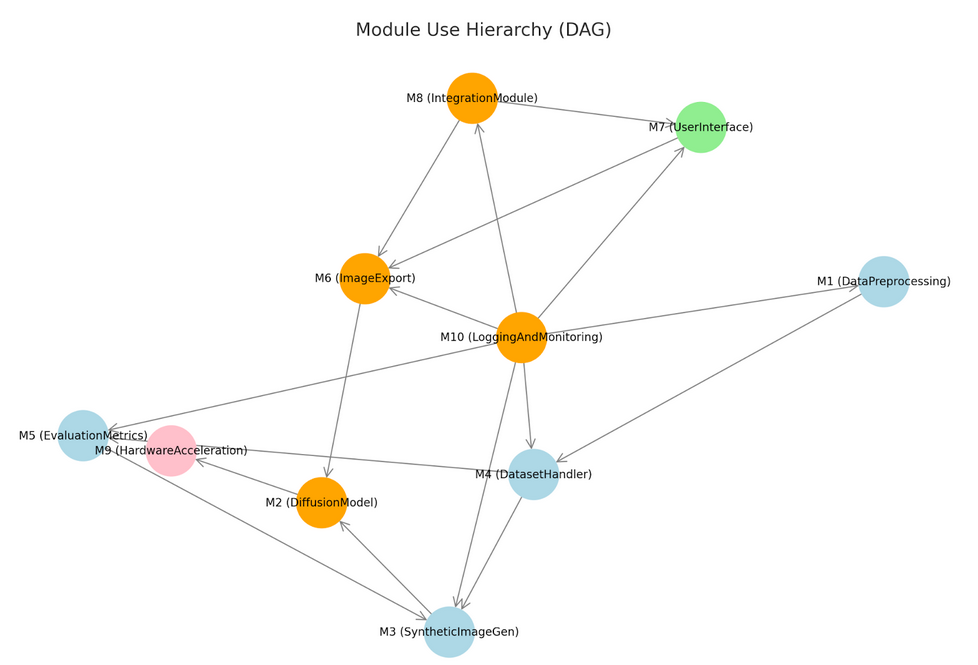
\includegraphics[width=10cm]{image}

The Directed Acyclic Graph (DAG) above visualizes the Use Hierarchy Between Modules based on the Model-View-Controller architecture and the provided module dependencies. Each node represents a module, and edges indicate usage relationships. Colors distinguish categories:
\begin{itemize}
\item Light Blue: Model modules
\item Light Green: View modules
\item Orange: Controller modules
\item Pink: Hardware modules
\end{itemize}



\section{User Interfaces}


\newpage{}

\end{document}